\documentclass[english,ngerman,paper=a5,headsepline=true,9pt,DIV=12,BCOR=0.7cm]{scrbook}
%
% explanation of options: the final version of the thesis is to be
% printed on a5 paper. It can also be printed on a4 paper using the
% «booklet» option. The advantage is, that the thesis will look on
% screen exactly as it will on paper. The thesis can also be printed
% on a5 printers in the copy shop of your liking.
%
% the language can be selected further down, the command is self
% explanatory. «headsepline» will result in a horizontal line in (below)
% the header.
%
% BCOR is the binding margin correction, it will increase the inner
% margin, so that binding can be done. No other geometry information
% is required.
%
% Our current IST binding procedure does not consume the inner margin
% much, so it appears that BCOR should be of size 0. But you might
% want to set it to a nonzero value if you prefer to gently open the
% booklet and not damage the back.

% important packages
%

\usepackage{typearea}           % recalculates the type area using the BCOR
                                % argument
\usepackage[utf8]{inputenc}     % text encoding in this file change to
                                % latin1 if you prefer that

\usepackage{lmodern}            % standard latex font

\usepackage[sc,osf]{mathpazo}   % the default font used in this
                                % manuscript (a bit thicker than
                                % lmodern), comment this package out
                                % if you want the default font

\usepackage[T1]{fontenc}        % internal LaTeX font management, important for letters like ä,ö etc.

\usepackage{babel}              % langauge related package


\usepackage{graphicx}           % to include graphics (pdflatex
                                % includes: png,pdf,jpg and more, but
                                % not eps! [nor ps])
\usepackage{amsmath,amssymb}    % math packages, e.g. for align and pmatrix environments
\usepackage{color}
\usepackage[usenames]{xcolor}   % you might consider using the dvipsnames option for more colors
\usepackage{tikz}               % graphics inside latex; very powerful
\usepackage{microtype}			% typographic enhancements
\usepackage{qrcode} 			% generating QR codes


% optional packages (but nice)
%
\usepackage{booktabs} % nice tables: \toprule, \midrule and \bottomrule
\usepackage{varioref} % references with pagenumbers, use \vref{«key»} for that; otherwise \ref and \eqref
\usepackage{icomma}   % if you write in german and have to
% use commas in numbers, this package
% will make everything right: 1,2 will not look like that: 1, 2 - while
% f(a, b) will have a small space between the function arguments


% even more optional packages
%
\usepackage{marginnote}         % e.g. for url on the side
\usepackage{cite}               % improved citation management for numerical citations,
\usepackage{listings}           % nicely formated code, see the
                                % packagae manual, good if you have to
                                % include programming code examples
\lstset{language=R,basicstyle=\ttfamily,frame=top} % an example setting for R code
\usepackage{caption}            % provides \captionof{figure}{...}
% makro (e.g. inside a center environement).  this is important for
% captions outside of floats like the «figure» environment

% some color definitions
\colorlet{lcolor}{blue!40!black}
\colorlet{ucolor}{magenta!40!black}
\colorlet{ccolor}{green!40!black}

\usepackage[colorlinks=true,%
            linkcolor=lcolor,%
            urlcolor=ucolor,%
            citecolor=ccolor]{hyperref} % makes references clickable
            % links will be in specified colors. You may set them to
            % black for final printing.



% template settings; makes things look nice, from a certain point of
% view.
%\flushbottom
\frenchspacing
\setcapindent{0em}
\addtokomafont{captionlabel}{\bfseries}
\pagestyle{headings}

% this will be decided by the advisor (the number of the thesis is
% internal to the institute)
\titlehead{Bachelor/\,Master Thesis 01 \hfill \raisebox{-4mm}{\includegraphics[height=12mm]{ist_logo}}}



% your settings:
%
\graphicspath{{figures/}{Figures/}{Abbildungen/}}  % this is where you store your figures, a list of folders

\subject{Subject} % if you see a purpose to that you can set a subject
\title{Master Thesis} % your title
%\subtitle{Systemtheorie und, oder Regelungstechnik} % more verbose title

% since we need the name of the author later on we define a variable
% for this purpose:
\newcommand{\authorstring}{Student 123} % replace «Student 123» with your name
\author{\authorstring}

\date{\today} % the submission date
\publishers{
  \begin{tabular}{rl}
    PrüferIn: & \emph{Prof.\,Dr. Prüfer}\\
    BetreuerIn: & \emph{Betreuername 1}\\
    &\emph{Betreuername 2}\\
  \end{tabular}\\[1cm]
  Institut für Systemtheorie und Regelungstechnik\\
  Universität Stuttgart\\Prof. Dr.-Ing. Frank Allg\"ower} % List your advisors and examinors here




% main document
%
% use the ususal KOMA script and LaTeX commands. Give some thought to
% your citation style and ask your advisor about that.  include
% appropriate packages and cite away...

\begin{document}
\selectlanguage{english}        % select ngerman if you want that
%\KOMAoptions{oneside} %% this didn't work, but maybe it will, when KOMAscript is updated
\KOMAoptions{twoside=false} % because we use the titlepage as the coverpage
\recalctypearea
\maketitle
\KOMAoptions{twoside=true} % and we switch back to twosided print
\recalctypearea

\tableofcontents


\chapter{Some Helpful Remarks}
The \texttt{mathpazo} font has a special property regarding numbers and
context: Text $1234$ 1234. An Example: In the year 1996 it was decided
that $\pi$ shall be exactly $3$. This way, numbers outside of a
mthematical context will not draw any attention to them as they look
like letters (1996), while math related numbers will (\verb|$1996$|
will result in $1996$). If you don't want this feature, remove the
\texttt{osf} option from the \texttt{mathpazo} package.

\section{On Citations}
\label{sec:citations}
The following was taken from the wikibook page on citations
(margin)$^]$. \marginnote{\rotatebox{90}{\url{http://en.wikibooks.org/wiki/LaTeX/Bibliography_Management}}}\\
\begin{minipage}{0.8\linewidth}
  \textbf{Sidenote}\qquad Consider using \texttt{QR} codes, if you
  want to link to something, in addition to \texttt{url}s. Another
  good practice is the use of the \texttt{hyperref} package. Note, that
  you can click on the \texttt{url} in the margin if you are viewing
  this on screen. %Finally, to achieve the same effect as in this
%  paragraph, you might want to consider the \texttt{wrapfig} package.
\end{minipage}
\vspace*{0.03\linewidth}
\begin{minipage}{0.17\linewidth}
  	\textcolor{black}{\qrcode[padding,height=0.9\linewidth]{http://en.wikibooks.org/wiki/LaTeX/Bibliography_Management}}
\end{minipage}

For any academic/research writing, incorporating
references into a document is an important task. Fortunately, LaTeX
has a variety of features that make dealing with references much
simpler, including built-in support for citing references. However, a
much more powerful and flexible solution is achieved thanks to an
auxiliary tool called BibTeX (which comes bundled as standard with
LaTeX).

BibTeX provides for the storage of all references in an external,
flat-file database. This database can be linked to any LaTeX document,
and citations made to any reference that is contained within the
file. This is often more convenient than embedding them at the end of
every document written. There is now a centralized bibliography source
that can be linked to as many documents as desired (write once, read
many!). Of course, bibliographies can be split over as many files as
one wishes, so there can be a file containing references concerning
General Relativity and another about Quantum Mechanics. When writing
about Quantum Gravity (QG), which tries to bridge the gap between
these two theories, both of these files can be linked into the
document, in addition to references specific to QG.

To actually cite a given document is very easy. Go to the point where
you want the citation to appear, and use the following:
\begin{verbatim}
\cite{cite_key},
\end{verbatim}
where the \texttt{cite\_key} is that of the bibitem you wish to
cite. When LaTeX processes the document, the citation will be
cross-referenced with the bibitems and replaced with the appropriate
number citation. The advantage here, once again, is that LaTeX looks
after the numbering for you. If it were totally manual, then adding or
removing a reference would be a real chore, as you would have to
re-number all the citations by hand.

I have previously introduced the idea of embedding references at the
end of the document, and then using the \verb|\cite{}| command to cite them
within the text. In this tutorial, I want to do a little better than
this method, as it's not as flexible as it could be. Which is why I
wish to concentrate on using BibTeX.

A BibTeX database is stored as a .bib file. It is a plain text file,
and so can be viewed and edited easily. The structure of the file is
also quite simple. An example of a BibTeX entry:
\begin{verbatim}
@article{greenwade93,
    author  = "George D. Greenwade",
    title   = "The {C}omprehensive {T}ex\
              {A}rchive {N}etwork ({CTAN})",
    year    = "1993",
    journal = "TUGBoat",
    volume  = "14",
    number  = "3",
    pages   = "342--351"
}
\end{verbatim}

Each entry begins with the declaration of the reference type, in the
form of \verb|@type|. BibTeX knows of practically all types you can think of,
common ones are: book, article, and for papers presented at
conferences, there is inproceedings. In this example, I have referred
to an article within a journal.

After the type, you must have a left curly brace `\{' to signify the
beginning of the reference attributes. The first one follows
immediately after the brace, which is the citation key, or the BibTeX
key. This key must be unique for all entries in your bibliography. It
is this identifier that you will use within your document to
cross-reference it to this entry. It is up to you as to how you wish
to label each reference, but there is a loose standard in which you
use the author's surname, followed by the year of publication. This is
the scheme that I use in this tutorial.

Next, it should be clear that what follows are the relevant fields and
data for that particular reference. The field names on the left are
BibTeX keywords. They are followed by an equals sign ($=$) where the
value for that field is then placed. BibTeX expects you to explicitly
label the beginning and end of each value. I personally use quotation
marks ("), however, you also have the option of using curly braces
(`\{', `\}'). But as you will soon see, curly braces have other roles,
within attributes, so I prefer not to use them for this job as they
can get more confusing. A notable exception is when you want to use
characters with umlauts (ü, ö, etc), since their notation is in the
format \verb|\"{o}|, and the quotation mark will close the one
opening the field, causing an error in the parsing of the
reference. Using \verb|\usepackage[utf8]{inputenc}| in the
preamble to the .tex source file can get round this, as the accented
characters can just be stored in the .bib file without any need for
special markup. This allows a consistent format to be kept throughout
the .bib file, avoiding the need to use braces when there are umlauts
to consider.

Remember that each attribute must be followed by a comma to delimit
one from another. You do not need to add a comma to the last
attribute, since the closing brace will tell BibTeX that there are no
more attributes for this entry, although you won't get an error if you
do.

It can take a while to learn what the reference types are, and what
fields each type has available (and which ones are required or
optional, etc). So, look at this entry type reference and also this
field reference for descriptions of all the fields. It may be worth
bookmarking or printing these pages so that they are easily at hand
when you need them.

\section{Math Symbols}
\label{sec:math}
A fraction is created using the \verb|\frac{numerator}{denominator}|
command. Likewise, the binomial coefficient (aka the Choose function)
may be written using the \verb|\binom| command:
\begin{align}
  \binom{n}{k}&=\frac{n!}{k!(n-k)!}\,, &\sum_{k=1}^n \binom{n}{k} \alpha^k \beta^k&=(\alpha+\beta)^n\,.  \label{eq:binomials}
\end{align}
The full command set for~\eqref{eq:binomials}:
\begin{verbatim}
\begin{align}
  \binom{n}{k}&=\frac{n!}{k!(n-k)!}\,, &
  \sum_{k=1}^n \binom{n}{k} \alpha^k \beta^k&=(\alpha+\beta)^n\,.
  \label{eq:binomials}
\end{align}
\end{verbatim}
Examples for matrices:
\begin{align*}
  \dot x&=
  \begin{pmatrix}
    \gamma&\beta\\
    -\beta&\gamma
  \end{pmatrix}x + \delta &
  \dot y&=
  \begin{bmatrix}
    \gamma&\beta\\
    -\beta&\gamma
  \end{bmatrix}y + \eta
\end{align*}
\begin{verbatim}
\begin{align*}
  \dot x&=
  \begin{pmatrix}
    \gamma&\beta\\
    -\beta&\gamma
  \end{pmatrix}x + \delta&
  \dot y&=
  \begin{bmatrix}
    \gamma&\beta\\
    -\beta&\gamma
  \end{bmatrix}y + \eta
\end{align*}
\end{verbatim}
To round things up, a drawing in \texttt{tikz} without using the
figure environment, so that the figure doesn't float:
\begin{center}
  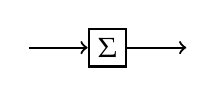
\begin{tikzpicture}[thick]
    \node (S) at (0,0) [draw,rectangle] {$\Sigma$};
    \draw[->]  (-1,0)  -- (S);
    \draw[->] (S) -- ++(1,0);
  \end{tikzpicture}
\captionof{figure}{a Ti\emph{k}Z example.}
\label{fig:system}
\end{center}
\begin{verbatim}
\begin{center}
  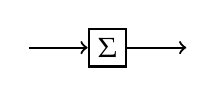
\begin{tikzpicture}[thick]
    \node (S) at (0,0) [draw,rectangle] {$\Sigma$};
    \draw[->]  (-1,0)  -- (S);
    \draw[->] (S) -- ++(1,0);
  \end{tikzpicture}
\captionof{figure}{a Ti\emph{k}Z example.}
\label{fig:system}
\end{center}
\end{verbatim}

Finally, a reference to the figure, to see whether it worked: see
Figure~\ref{fig:system}.

%failsafe text:
\chapter*{Eigenst\"{a}ndigkeitserkl\"{a}rung}
\selectlanguage{ngerman}
  Ich versichere hiermit, dass ich, \authorstring{}, die vorliegende
  Arbeit selbstst\"{a}ndig angefertigt, keine anderen als die
  an\-ge\-ge\-benen Hilfsmittel benutzt und sowohl w\"{o}rtliche, als auch
  sinngem\"{a}{\ss} entlehnte Stellen als solche kenntlich gemacht
  habe. Die Arbeit hat in gleicher oder \"{a}hnlicher Form noch keiner
  anderen Pr\"{u}fungsbeh\"{o}rde vorgelegen. Weiterhin best\"{a}tige ich, 
  dass das elektronische Exemplar mit den anderen Exemplaren \"{u}bereinstimmt.

\vspace{1cm}
\noindent{}\rule{0.39\textwidth}{0.4pt} \hspace{1.9cm} \rule{0.39\textwidth}{0.4pt}

\noindent{}Ort, Datum  \hspace{4.3cm} Unterschrift

%
% \bibliographystyle{alpha}
% \bibliographystyle{plain}
% \bibliography{mybibtexfile}
\end{document}
